\chapter{Cost Model Spreadsheets}\label{app:B_cost_model_spreadsheets}

\section{Static NPV Model}\label{app:B_static_model}
The static model described in Section \ref{ch4:cm_concept} was implemented in Microsoft Excel as a single sheet for cost analysis. Figures \ref{fig:static_model_sheet1} and \ref{fig:static_model_sheet2} show the model when flow rate is pre-defined and capacity depends on the input temperature of the produced brine. Not shown is the supporting look-up table for the EIA STEO-based electricity price forecast (Figure \ref{fig:electricity_pricing}).
\vfill
\pagebreak

\begin{figure}[H]
\centering
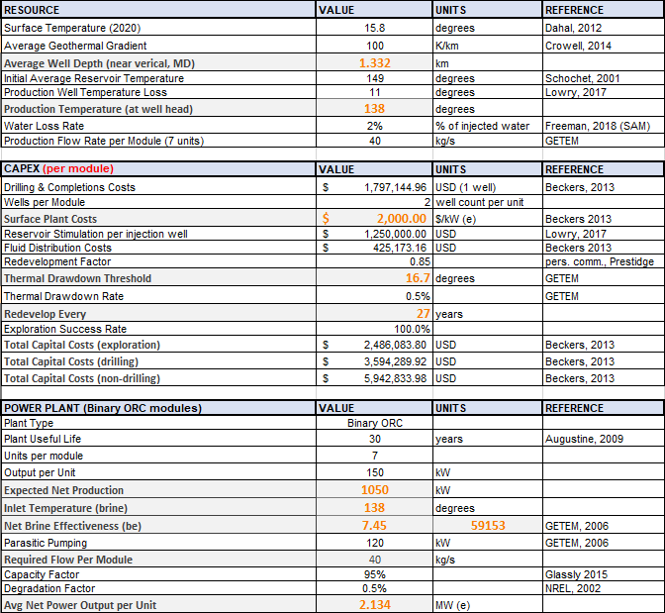
\includegraphics[width=\textwidth]{templates/images/Figure-Static_Model_SheetA.png}
\caption[Static cost model worksheet (part 1)]{First part of geothermal power plant expansion static NPV cost model.}
\label{fig:static_model_sheet1}
\end{figure}

\begin{figure}[H]
\centering
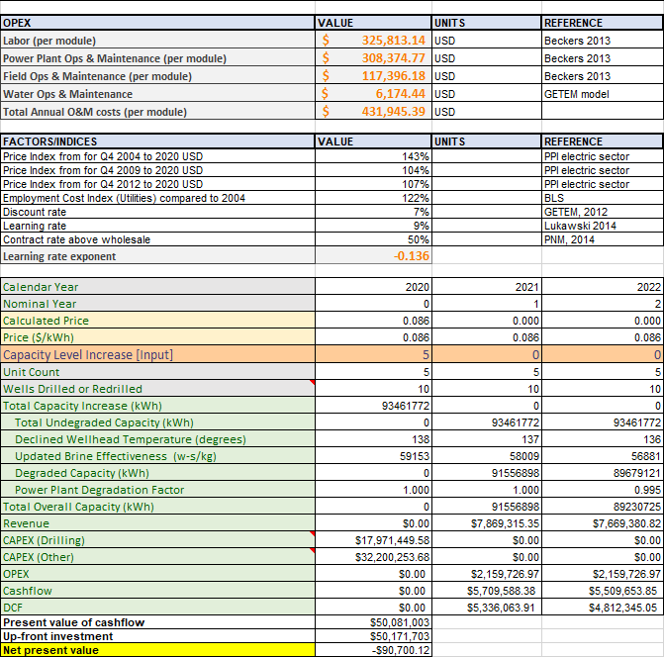
\includegraphics[width=\textwidth]{templates/images/Figure-Static_Model_SheetB.png}
\caption[Static cost model worksheet (part 2)]{Second part of geothermal power plant expansion static NPV cost model. The yearly breakdown of cost and revenue only extends out to year 2 for visualization purposes but continues to year 30 in the actual spreadsheet.}
\label{fig:static_model_sheet2}
\end{figure}
\pagebreak
\section{Flexible NPV Models}\label{app:B_flex_models}

\textbf{TO BE ADDED}